\documentclass{article}

\usepackage[final]{neurips}

\usepackage{multicol}
\usepackage{float}
\usepackage[center]{caption}

\usepackage[utf8]{inputenc} % allow utf-8 input
\usepackage[T1]{fontenc}    % use 8-bit T1 fonts
\usepackage{hyperref}       % hyperlinks
\usepackage{url}            % simple URL typesetting
\usepackage{booktabs}       % professional-quality tables
\usepackage{amsfonts}       % blackboard math symbols
\usepackage{nicefrac}       % compact symbols for 1/2, etc.
\usepackage{microtype}      % microtypography
\usepackage{graphicx}
\usepackage{amsmath}
\usepackage{xepersian}

\settextfont{XB Yas.ttf}

\title{
تمرین دوم
}


\author{%
  امیرحسین مهدی‌نژاد\\
  شماره دانشجویی 810800058\\
  \texttt{mahdinejad@ut.ac.ir} \\
}

\begin{document}


\begin{minipage}{0.1\textwidth}% adapt widths of minipages to your needs

\includegraphics[width=1.1cm]{Photos/UT_logo.png}
\end{minipage}%
\hfill%
\begin{minipage}{0.9\textwidth}\raggedleft
دانشکده فنی، دانشگاه تهران\\
الگوریتم‌های تصادفی -  
اسفند
ماه 1400\\
\end{minipage}
% \end{}

\makepertitle

% ----------------------------------------------------------------------
\section*{1}
فرض کنیم
$v_1, v_2, ..., v_n$
مقادیر مشاهده شده باشند. در نظر بگیریم
$V_t$
متغیر تصادفی باشد که در لحظه‌ی
$t$
مقدار داخل حافظه را نشان دهد.

اثبات استقرایی: بدیهی است برای حالت
$t = 1$
با احتمال یک، مقادیر
$v_1$
و
$V_t$
برابرند.

اگر برای هر
$1 \leq i \leq t$
مقدار
$P(V_t = v_i) = \frac{1}{t}$
باشد، در زمان
$t+1$
با احتمال
$\frac{1}{t+1}$
داریم
$V_{t+1} = v_{t+1}$:
$$ P(V_{t+1} = v_{t+1}) = \frac{1}{t+1} $$
احتمال اینکه جابجایی در زمان 
$t$
انجام نشده باشد را در احتمال قبلی ضرب می‌کنیم:
$$ P(V_{t+1} = v_i) = P(\text{\lr{no change at t}}) \times P(V_t = v_i) = \frac{t}{t+1} \times \frac{1}{t} $$
\rule{\linewidth}{1pt}
% ----------------------------------------------------------------------
\section*{2}
\subsection*{a}
با توجه به بند آخر صورت سوال، توزیع برنولی با احتمال
$p$
در نظر می‌گیریم که مثبت شدن یک تست از
$k$
تست با احتمال
$ P(\text{problem}_{2.a}) = 1 - (1 - p)^k $
رخ می‌دهد.

\subsection*{b}
برای هرکدام از گروه‌های
$k$
نفره، اگر کسی مثبت نباشد یک تست کافیست وگرنه به
$k+1$
تست نیاز داریم. برای کل
$n$
نفر، امید ریاضی تعداد تست‌های مورد نیاز برابر خواهد بود با:
$$E(X) = \frac{n}{k}\left( (1-p)^k + (k+1) \times \left( 1 - (1 - p)^k \right) \right)$$

\subsection*{c}
در واقع به دنبال
$k$
ای هستیم که تعداد تست‌های مورد نیاز را کمینه کند.
$$ E(X) = n \left( \frac{k}{k+1} - (1 - p)^k \right) $$
از رابطه‌ی بالا مشتق می‌گیریم:
$$\frac{\partial E}{\partial k} = n \left(- \frac{1}{k^2} + \log(\frac{1}{1-p}) \times (1-p)^k \right)$$
با صفر قرار دادن این عبارت می‌توان مقدار بهینه را بدست آورد. (تقریبا
$\frac{1}{\sqrt{p}}$
)

\subsection*{d}
$$\frac{n}{k} + n - n(1-p)^k < n \xrightarrow{} \frac{1}{k} < (1-p)^k \xrightarrow{} - \frac{\ln k}{k} < \ln(1-p) \xrightarrow{} p < 1 - e^{- \frac{\ln k}{k}} = 1 - k^{- \frac{1}{k}}$$

هرچقدر
$p$
به صفر نزدیک‌تر باشد، مقدار
$k$
بهینه بیشتر می‌شود. هرچقدر تست ما کمتر نتیجه‌ی مثبت بدهد، آزمایش توده‌ای به‌صرفه‌تر خواهد بود.

از طرفی هرچه
$p$
به یک نزدیک‌تر باشد، مقدار
$k$
بهینه کمتر خواهد بود.

\rule{\linewidth}{1pt}
% ----------------------------------------------------------------------
\section*{3}

در هر بازی احتمال برد
$\frac{1}{2}$
است.

با فرض اینکه در
$k-1$
بازی نخست باخته باشیم و در بازی
$k$
ام ببریم، پول بدست آمده از این قرار خواهد بود:
$$-1-2-...-2^{k-2}+2^{k-1} = 1$$
پس در نهایت با ۱ دلار بیشتر از پولی که ابتدا داشتیم، خارج می‌شویم. احتمال اینکه این اتفاق بیوفتد:
$\sum^{\infty}_{i=1}\frac{1}{2^i} = 1$

می‌خواهیم نشان دهیم میزان پول مورد انتظاری که باید داشته باشیم بی‌نهایت است. بیشترین مقدار باخت برابر با
$2^{k-1} - 1$
خواهد بود. لذا احتمال باخت
$k-1$
راند و بردن راند
$k$
ام را در آن ضرب می‌کنیم:
$$E[X] = \sum^{\infty}_{i=1} \left(\frac{1}{2^i} \times \left(2^{i-1}-1\right) \right) = \sum^{\infty}_{i=1} \frac{1}{2} - \sum^{\infty}_{i=1} \frac{1}{2^i} = \infty$$
\rule{\linewidth}{1pt}
% ----------------------------------------------------------------------

\section*{4}
فایل
\lr{perm.cpp}
ضمیمه‌ی این گزارش شده و کدهای مربوطه به صورت توابع جداگانه در آن پیاده‌سازی شده است.

\subsection*{a}
در تابع
\lr{perm\_nlogn}
ابتدا یک وکتور از زوج‌مرتب‌های
\lr{<int, int>}
تعریف شده است که در درایه‌های
\lr{first}
مقادیر رندوم و در درایه‌های
\lr{second}
آن، اعداد ۱ تا
\lr{n}
را قرار دادیم.

با مرتب‌سازی وکتور مذکور بر اساس مقادیر
\lr{first}
طبیعتا یک جایگشت از اعداد ۱ تا
\lr{n}
در مقادیر
\lr{second}
خواهیم داشت.
\begin{figure}[H]
    \centering
    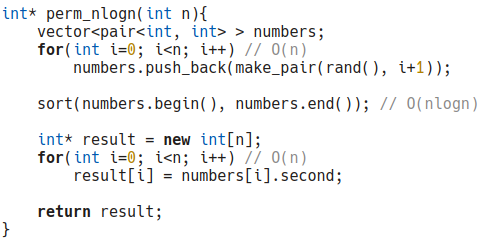
\includegraphics[width=0.5\linewidth]{Photos/HW2/a.png}
    \caption{
    پیاده‌سازی بند
    \lr{a}
    از مرتبه‌ی
    \lr{nlogn}
    }
    \label{fig:my_label}
\end{figure}

\subsection*{b}
در تابع
\lr{perm\_n}
ابتدا آرایه با اعداد ۱ تا
\lr{n}
پر می‌شود و سپس به سبک مرتب‌سازی انتخابی یک عنصر به جایگاه خودش منتقل می‌شود. این بار بجای اینکه مینی‌مم یا ماکزیمم پیدا شود، عنصری رندوم را با استفاده از تابع رندومی که در اختیارمان قرار گرفته انتخاب می‌کنیم.

با توجه به اینکه هر جایگشتی را با استفاده از مرتب‌سازی انتخابی می‌توان مرتب کرد، خروجی تابع پیاده‌سازی شده نیز حتما یک جایگشت از اعداد ۱ تا
\lr{n}
خواهد بود.
\begin{figure}[H]
    \centering
    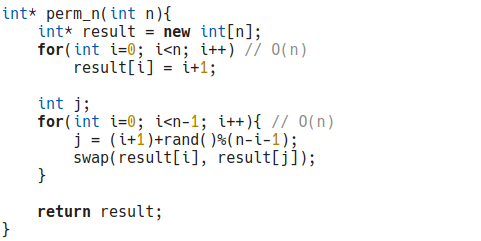
\includegraphics[width=0.5\linewidth]{Photos/HW2/b.png}
    \caption{
    پیاده‌سازی بند
    \lr{b}
    از مرتبه‌ی
    \lr{n}
    }
    \label{fig:my_label}
\end{figure}

\subsection*{c}
در تابع
\lr{perm\_k}
یک
\lr{map}
از اعداد داریم و با
\lr{k}
بار پیمایش، هر سری یک عدد رندوم از ۱ تا
\lr{n}
تولید کرده و در صورتی که قبلا در
\lr{map}
نبوده، آن را اضافه می‌کنیم.

در نهایت
\lr{k}
عدد خواهیم داشت که جایگشتی از
\lr{k}
تا از اعداد ۱ تا
\lr{n}
خواهد بود. گرچه چک کردن وجود هر عنصر از مرتبه‌ی ۱ است ولی با توجه به حلقه‌ی
\lr{while}
داخلی، استفاده از این روش در صورتی که 
$k > \frac{n}{2}$
باشد، معقول نیست.
\begin{figure}[H]
    \centering
    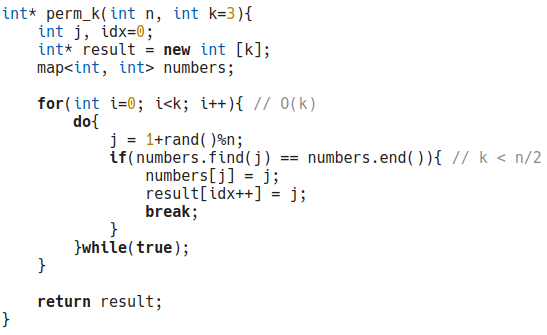
\includegraphics[width=0.6\linewidth]{Photos/HW2/c.png}
    \caption{
    پیاده‌سازی بند
    \lr{c}
    از مرتبه‌ی
    \lr{k}
    }
    \label{fig:my_label}
\end{figure}

\end{document}